\title{CS289 Initial Report: \\
Methods of handling missing data for classification
\vspace{15mm}}

\author{Rafael Valle\thanks{\href{mailto:rafaelvalle@berkeley.com}{\nolinkurl{rafaelvalle@berkeley.com}}.} \hspace{10mm}
Jason Poulos\thanks{\href{mailto:poulos@berkeley.edu}{\nolinkurl{poulos@berkeley.edu}}.}
\vspace{15mm}}

\date{\today}

%%%%%%%%%%%%%%%%%%%%%%%%%%%%%%%%%%%%%%%%%%%%%%%%%%
% Set document class
\documentclass[12pt]{article}

% Define packages
\usepackage{graphicx,amsfonts,psfrag,layout,subcaption,array,longtable,lscape,booktabs,dcolumn,natbib,amsmath,amssymb,amssymb,amsthm,setspace,epigraph,chronology,color, colortbl,caption,wasysym}
\usepackage[]{graphicx}\usepackage[]{color}
\usepackage[page]{appendix}
\usepackage{hyperref, url}
\usepackage[section]{placeins}
\usepackage[linewidth=1pt]{mdframed}
\usepackage[margin=1in]{geometry} %1 inch margins

% Footnotes stick at the bottom
\usepackage[bottom]{footmisc}

% New footnote characters
\usepackage{footmisc}
\DefineFNsymbols{mySymbols}{{\ensuremath\dagger}{\ensuremath\ddagger}\S\P
   *{**}{\ensuremath{\dagger\dagger}}{\ensuremath{\ddagger\ddagger}}}
\setfnsymbol{mySymbols}

% New tabular environment
\usepackage{tabularx}
\newcolumntype{Y}{>{\raggedleft\arraybackslash}X}% raggedleft column X

% Define appendix
\renewcommand*\appendixpagename{Appendix}
\renewcommand*\appendixtocname{Appendix}

% Position floats
\renewcommand{\textfraction}{0.05}
\renewcommand{\topfraction}{0.95}
\renewcommand{\bottomfraction}{0.95}
\renewcommand{\floatpagefraction}{0.35}
\setcounter{totalnumber}{5}

% Colors for highlighting tables
\definecolor{Gray}{gray}{0.9}

% Different font in captions
\newcommand{\captionfonts}{\scriptsize}

\makeatletter  % Allow the use of @ in command names
\long\def\@makecaption#1#2{%
  \vskip\abovecaptionskip
  \sbox\@tempboxa{{\captionfonts #1: #2}}%
  \ifdim \wd\@tempboxa >\hsize
    {\captionfonts #1: #2\par}
  \else
    \hbox to\hsize{\hfil\box\@tempboxa\hfil}%
  \fi
  \vskip\belowcaptionskip}
%\makeatother   % Cancel the effect of \makeatletter

% Set Spacing
%\doublespacing

%Theorem
\newtheorem{theorem}{Theorem}

% Number assumptions
\newtheorem*{assumption*}{\assumptionnumber}
\providecommand{\assumptionnumber}{}
\makeatletter
\newenvironment{assumption}[2]
 {%
  \renewcommand{\assumptionnumber}{Assumption #1}%
  \begin{assumption*}%
  \protected@edef\@currentlabel{#1}%
 }
 {%
  \end{assumption*}
 }
\makeatother

% Macros
\newcommand{\Adv}{{\mathbf{Adv}}}
\newcommand{\prp}{{\mathrm{prp}}}                  % How to define new commands
\newcommand{\calK}{{\cal K}}
\newcommand{\outputs}{{\Rightarrow}}
\newcommand{\getsr}{{\:\stackrel{{\scriptscriptstyle\hspace{0.2em}\$}}{\leftarrow}\:}}
\newcommand{\andthen}{{\::\;\;}}    %  \: \; for thinspace, medspace, thickspace
\newcommand{\Rand}[1]{{\mathrm{Rand}[{#1}]}}       % A command with one argument
\newcommand{\Perm}[1]{{\mathrm{Perm}[{#1}]}}
\newcommand{\Randd}[2]{{\mathrm{Rand}[{#1},{#2}]}} % and with two arguments
\newcommand{\E}{\mathrm{E}}
\newcommand{\ind}{\mathbb{I}} % Indicator function
\newcommand{\pr}{\mathbb{P}} % Generic probability
\newcommand{\ex}{\mathbb{E}} % Generic expectation
\newcommand{\Var}{\mathrm{Var}}
\newcommand{\Cov}{\mathrm{Cov}}
\newcommand{\cov}{\mathrm{Cov}}
\DeclareMathOperator*{\plim}{plim}
\newcommand\independent{\protect\mathpalette{\protect\independenT}{\perp}}
\def\independenT#1#2{\mathrel{\rlap{$#1#2$}\mkern2mu{#1#2}}}
\newcommand{\possessivecite}[1]{\citeauthor{#1}'s [\citeyear{#1}]}
\newcommand{\todo}[1]{{\color{red}{TO DO: \sc #1}}}

\begin{document}

\maketitle

\section{Motivation}

Methods of handling missing data for neural networks classification model

Given that we plan to use NNets for income prediction ($income \geq \$ 50K/yr$) on the Adult dataset, we must handle missing data. This is less problematic for ML models such as random forest, decision trees, etc.

%Include necessary ?background? information:
  % What is the application domain and/or field of research?
  % Why is the problem important?
  % What specific questions are you trying to answer?

Item nonresponse is a common problem in survey data in several domains. Several techniques for data imputation (replace missing values with plausible ones) and direct estimation(all missing data is analyzed using a maximum likelihood approach) have been developed \cite{de2003prevention}.

Proper statistical adjustement of missing data is very important, as naive solutions might introduce bias. We're interested in using the data to train neuronal networks. This must be taken into account becouse higher input values will result in a higher activation input.

In this project, we plan to evaluate different data imputation and direct estimation techniques within the context of using a neural network income classifier on the ADULT dataset. We plan to compare our results to previous techniques and models, such as bla bla bla, that addressed this same question.

\section{Data}

%Talk about what data sources you are planning to use, including number of samples and number of features (if it's visual data -- include a sample).

We plan to experiment with the Adult dataset from the UCI Machine Learning Repository \citep{Lichman2013}. The dataset has 48,842 samples ($\mathrm{train}=32,561$ and $\mathrm{test}=1,6281$). The dataset contains 14 features: 6 continuous and 8 categorical. The prediction task is to determine whether a person makes over \$50,000 a year; 24\% of individuals in the training data make more than this amount. \\

Table \ref{benchmarks} shows the test error rates obtained by the data set donor \citep{kohavi1996}. All error rates were obtained after removing samples with missing values. The error rate to beat is 14.05\%. \\

Given the results of our experiments and if time permits, we may move to a much larger dataset, such as the 1940 full--count U.S. Census file \citep{napp2008, ruggles2010}. The 1940 Census has about 100 million samples and 100 features. 

\begin{table}[htb]
\centering
\begin{tabular}{@{}ll@{}}
\toprule
\textbf{Algorithm}       & \textbf{Error} \\ \midrule
1  C4.5                  & 15.54          \\
2  C4.5-auto             & 14.46          \\
3  C4.5 rules            & 14.94          \\
4  Voted ID3 (0.6)       & 15.64          \\
5  Voted ID3 (0.8)       & 16.47          \\
6  T2                    & 16.84          \\
7  1R                    & 19.54          \\
8  NBTree                & 14.10          \\
9  CN2                   & 16.00          \\
10 HOODG                 & 14.82          \\
11 FSS Naive Bayes       & 14.05          \\
12 IDTM (Decision table) & 14.46          \\
13 Naive-Bayes           & 16.12          \\
14 Nearest-neighbor (1)  & 21.42          \\ \bottomrule
\end{tabular}
\caption{Test set error rates on Adult dataset for various algorithms, obtained after removal of samples with missing values and using the original train/test split. Source: \citet{Lichman2013}.}
\label{benchmarks}
\end{table}

\subsection{Patterns of missing values}

The Adult dataset has 3,620 (7.4\%) samples containing missing values. Missing values occur in three of the categorical features: \textit{Work class}, \textit{Occupation}, and \textit{Native country}. It is unlikely that these values are missing completely at random (MCAR); it is more likely, and much less desirable that the values are not missing at random (MNAR). Since these data originate from a survey, the missing values may be due to respondents unwilling or unable to provide an answer.  \\

Uncovering patterns of missing values in the dataset will help select strategies for imputing missing values. The histogram (left) in Figure \ref{proportion-missing} shows \textit{Work class} and \textit{Occupation} each have about 5.6\% of missing values, and \textit{Native country} has about 1.7\% missing values. The aggregation plot (right) shows 5.5\% of samples are missing values for both \textit{Work class} and \textit{Occupation}. Less than 2\% of samples are missing just \textit{Native country} and less than 1\% are missing all three features.

\begin{figure}[htbp] 
   \centering
   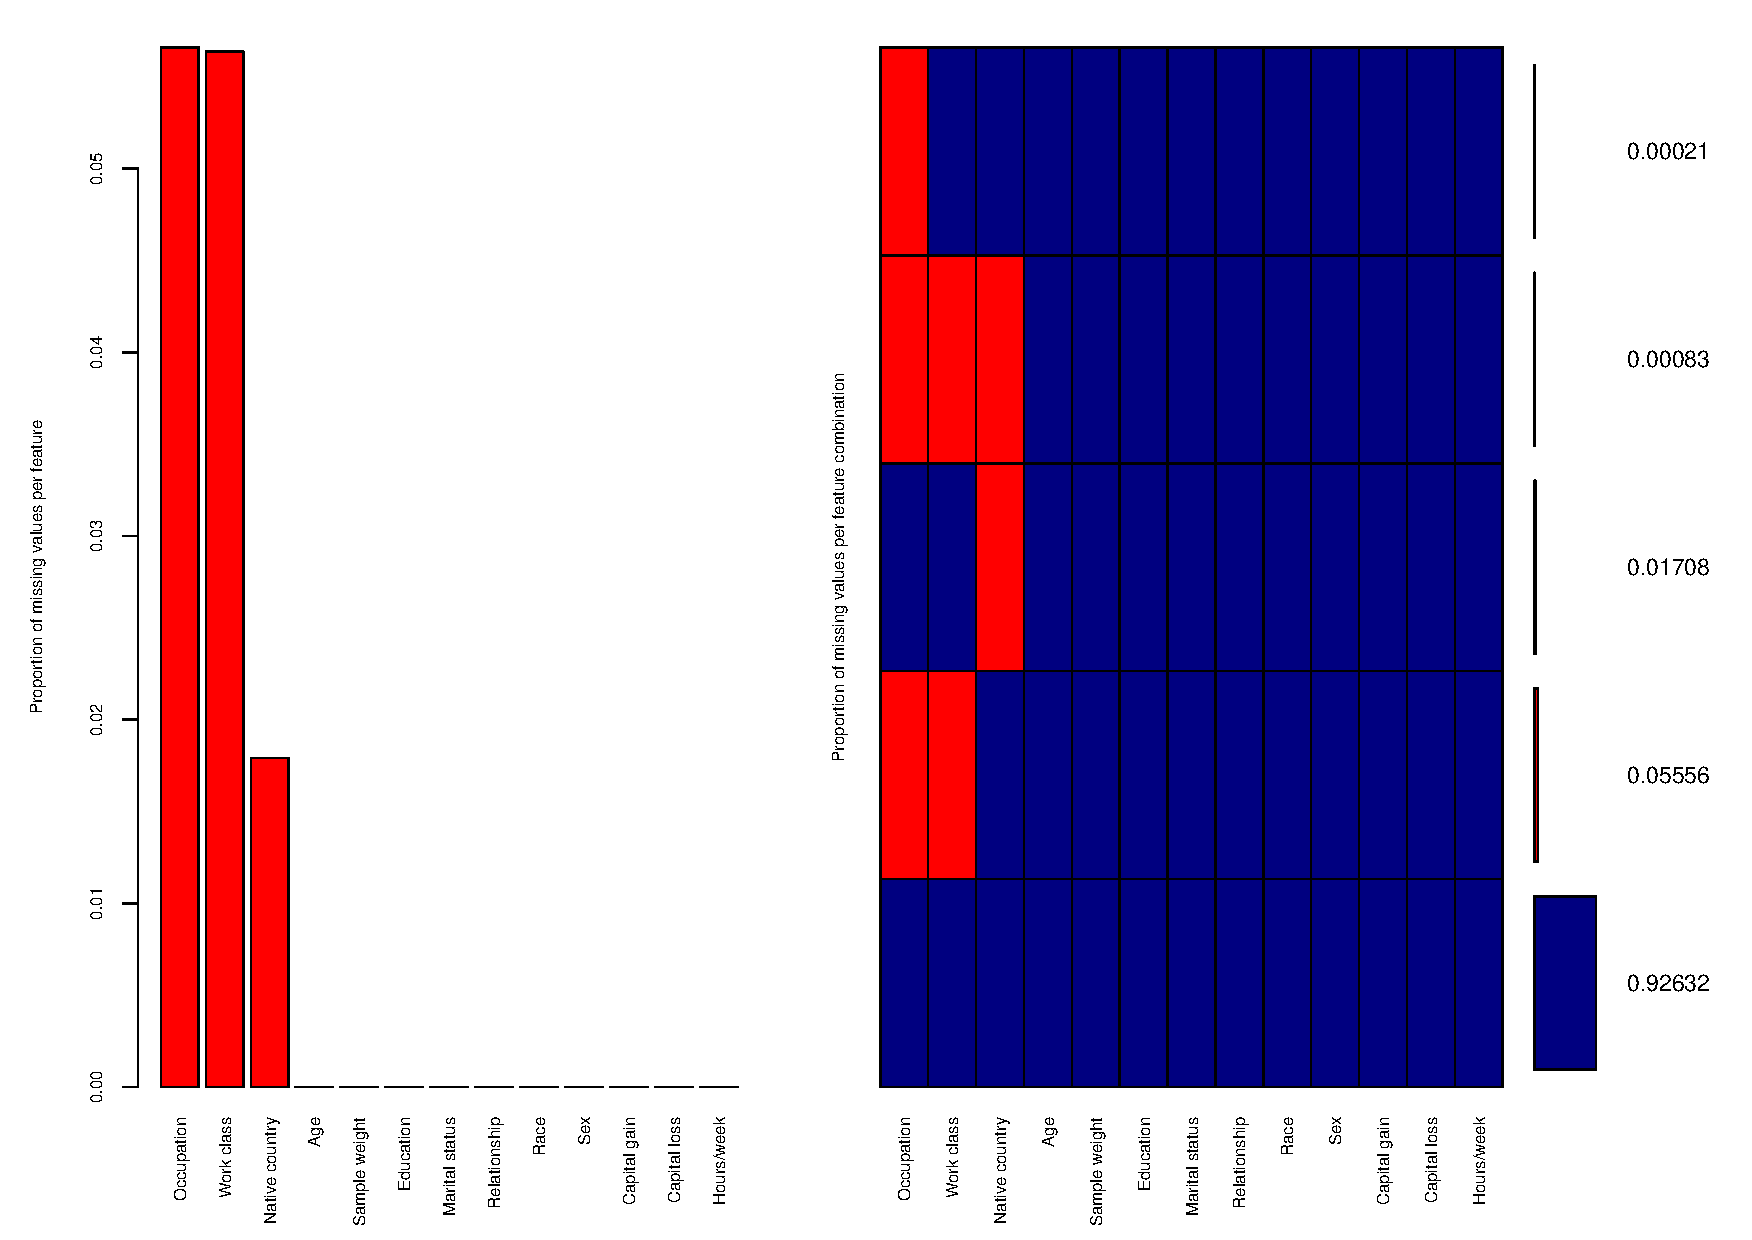
\includegraphics[scale=0.6]{proportion-missing.pdf} 
   \caption{Histogram of proportion of missing values in each feature (Left) of Adult training set and aggregation plot of all existing combinations of missing and non-missing values in the samples (Right).}
   \label{proportion-missing}
\end{figure}

%\begin{figure}[htbp] 
%   \centering
%   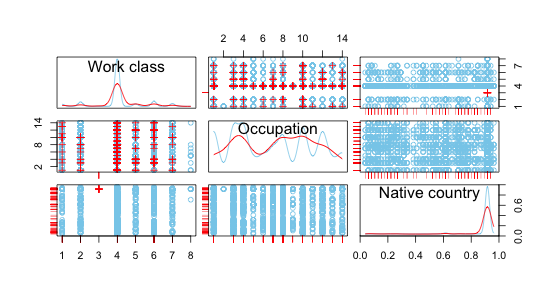
\includegraphics[scale=1]{scatter-matrix-missing.png} 
%   \caption{Scatterplot Matrix of features with missing values in Adult training set. Blue represents observed values and red represents missing values.}
%   \label{scatter-matrix-missing}
%\end{figure}

\begin{figure}[htbp] 
   \centering
   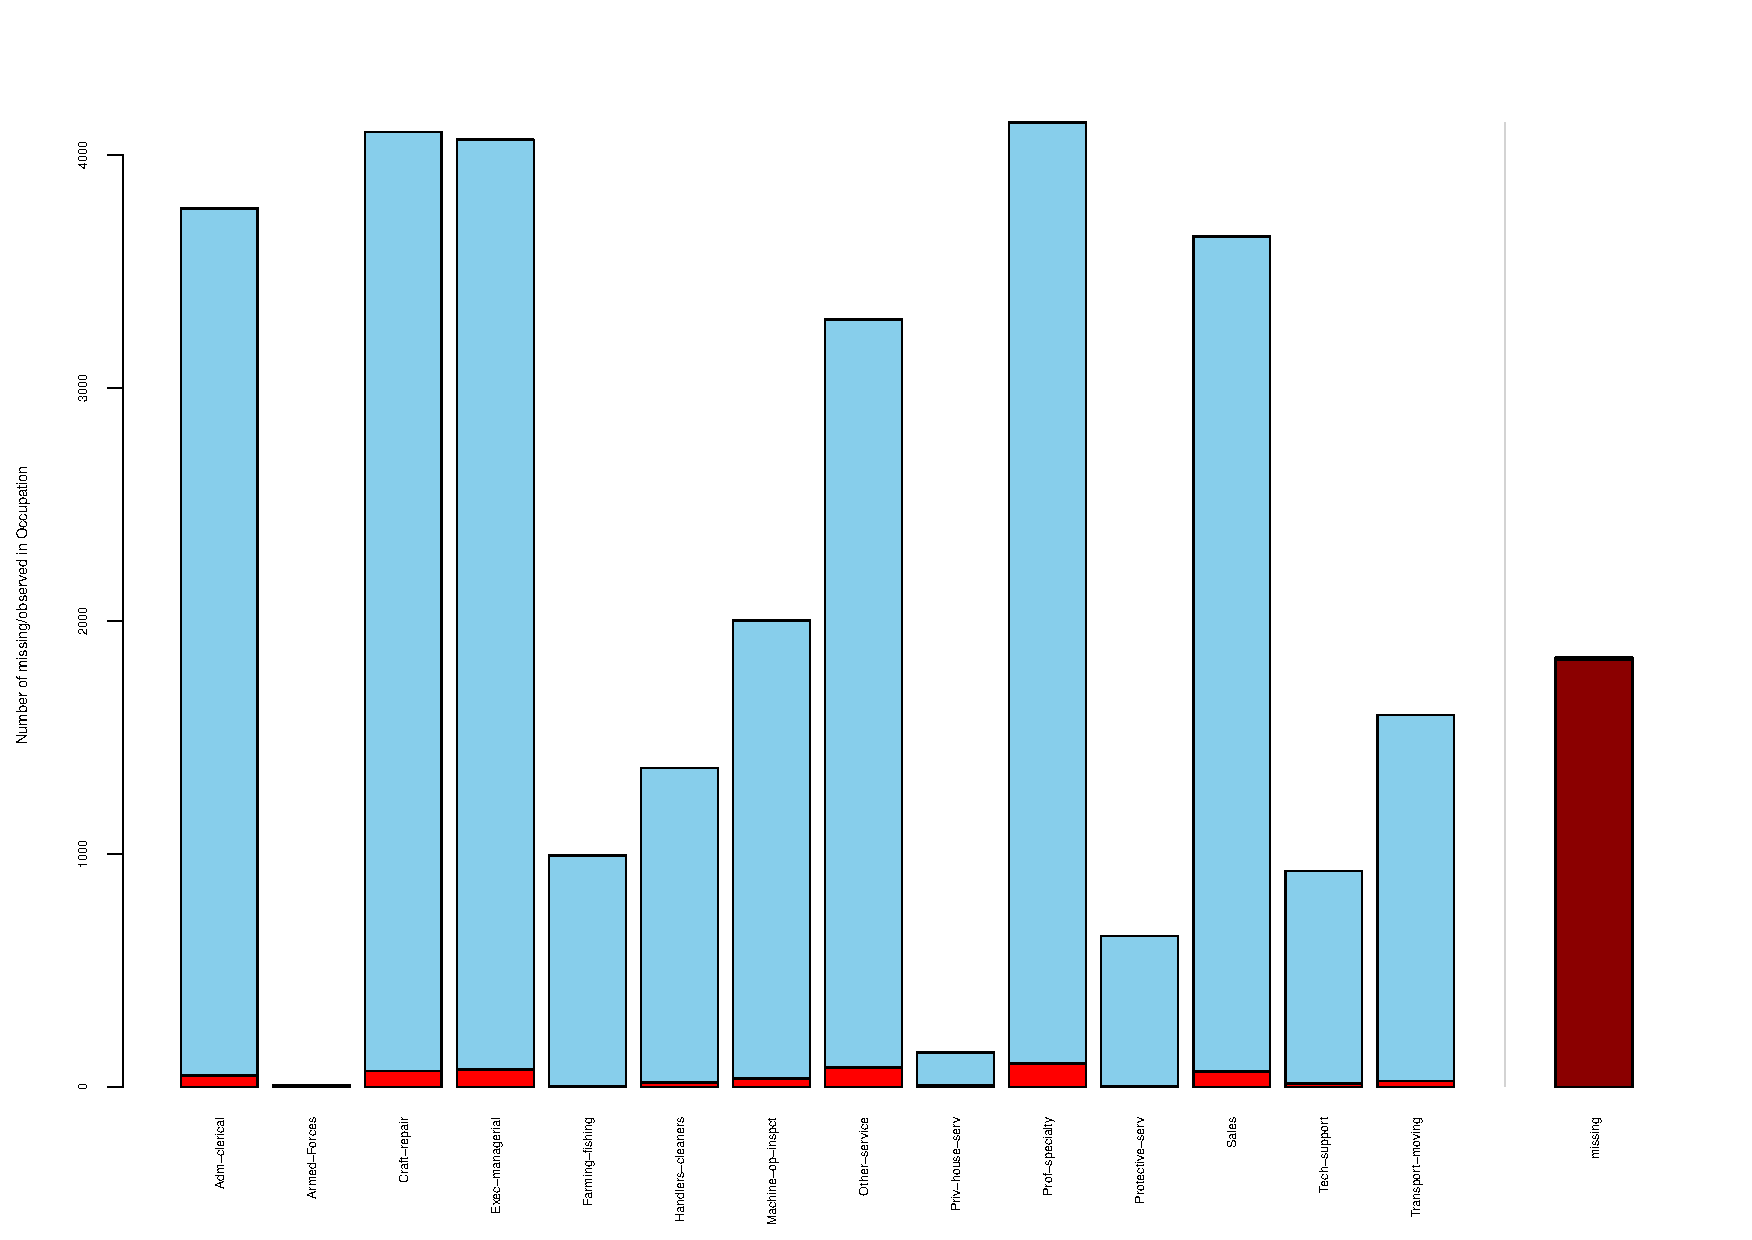
\includegraphics[scale=0.6]{barplot-occ-missing.pdf} 
   \caption{Barplot of the feature \textit{Occupation} in the Adult training set (blue). Imputed values in \textit{Work class} or \textit{Native country} are highlighted in red.}
   \label{barplot-occ-missing}
\end{figure}

\section{Methods}

% Explain which methods you are planning to use and why.

\subsection{Techniques for handling missing data}
Assuming that the techniques below are easy to implement, we would like to compare their efficiency in imputing the missing values.

\begin{enumerate}
\item Basic Statistics : Replace the missing data with the mean or median of the feature vector. This is the most naive approach and since the missing variables in the ADULT dataset are all categorical, using the mean is not appropriated.
\item One-hot : Create an binary variable to indicate whether or not a specific feature is missing. This technique was mentioned by Isabelle
\item Nearest Neighbor Imputation : Recursively compute the K-Nearest Neighbors of the observation with missing data and assign median of the K-neighbors to the missing data. This technique is used in airbnb's fraud detection algorithm and explained in their website.
\item Logistic Regression : train a logistic regression model with all features except the feature with the missing variable to predict the missing value.
\item Bagging : Use one bag tree model for each predictor based on all other
   predictors.
\item Factor analysis : Perform some sort of factorization on the design matrix, project the design matrix onto the first two eigen vectors and replace the missing values by the values that might be given by the projected design matrix.
\item Find other features with distribution similar to the feature containing missing data and use this information (e.g. correlation) to fill in in the missing data. However, if two features are highly correlated, it might be better to remove one of them.
\end{enumerate}

\subsection{Neural networks for classification}

\pagebreak

%Bibliography
\bibliographystyle{plainnat}
\bibliography{refs}

%%Appendix
%\pagebreak
%\begin{appendices}
%
%\begin{figure}[htbp]
%\begin{center}
%\includegraphics[width = 1\textwidth]{rmse_ratec_rates}
%\caption{Simulated RMSE, binned by compliance rate and percent eligible for the RCT. Darker tiles correspond to worse estimates of PATT.}
%\label{fig:sim_tiles}
%\end{center}
%\end{figure}
%
%\end{appendices}

\itemize
\end{document}


